\section{Introduction}

\section{Numerical Simulations - Avellaneda \& Stoikov}

\begin{lstlisting}[language=Python, caption=Auxiliary Functions]
import numpy as np
        
def computeReservePrice(s,q,gamma,sigma,t,T):
    return s-q*gamma*(sigma**2)*(T-t)

def computeSpread(gamma,sigma,t,T,k):
    return (gamma * (sigma ** 2) * (T-t)) + ((2 / gamma) * 
        np.log(1 + (gamma / k)))

def computeRate(A,k,delta):
    return A*np.exp(-k*delta)

def computeSamplePath(S0, sigma, dt, T):
    return np.insert(S0 + np.cumsum(sigma * np.sqrt(dt) * 
        np.random.choice([1,-1], int(T/dt))), 0, S0)
\end{lstlisting}

\texttt{computeReservePrice} takes the current stock price, current
inventory, risk aversion, volatility, current time and end time as
arguments and returns the current reservation price as given in 
(\ref{eq:3.34}).

\texttt{computeSpread} takes the risk aversion, volatility, current
time, end time and orderbook parameter $k$ as arguments and computes
the current spread as given by (\ref{eq:3.35}).

\texttt{computeRate} computes the function $\lambda$ in the form assumed
by (\ref{eq:3.24}), taking the orderbook parameters $A$ and $k$ and the 
current spread $\delta$ as arguments.

\texttt{computeSamplePath} generates a sample path from a brownian motion
from $t$ to $T$ with stepsize $\mathrm dt$, volatility $\sigma$ and starting
value $S_0$.

\newpage
\begin{lstlisting}[language=Python, caption=Avellaneda-Stoikov Model]
def simulateBothStrategies(gamma):
S0=100
T=1
sigma=2
dt=0.005
inv_q=0
sym_q=0
k=1.5
A=140
inv_X=0
sym_X=0
inf_X=0

inv_bids = []
inv_asks = []
inv_wealth = []
inv_adj_wealth = []
inv_inventory = []

sym_bids=[]
sym_asks=[]
sym_wealth = []
sym_adj_wealth = []
sym_inventory = []

price_process = computeSamplePath(S0, sigma, dt, T)

sym_spread = 0
for i in np.arange(0, T, dt):
    sym_spread += computeSpread(gamma, sigma, i, T, k)
av_sym_spread = (sym_spread / (T / dt))
sym_prob = min(A * np.exp(- k * av_sym_spread / 2) * dt, 1)
sym_bids = price_process - av_sym_spread/2
sym_asks = price_process + av_sym_spread/2

for step, s in enumerate(price_process):
    r = computeReservePrice(s,inv_q,gamma,sigma,step*dt,T)
    spread = computeSpread(gamma,sigma,step*dt,T,k)/2
    delta_a = (spread+r)-s
    delta_b = s-(r-spread)

    inv_asks.append(s+delta_a)
    inv_bids.append(s-delta_b)
    inv_wealth.append(inv_X)
    inv_adj_wealth.append(inv_X+inv_q*s)
    inv_inventory.append(inv_q)

    prob_a = min(computeRate(A,k,delta_a)*dt, 1)
    prob_b = min(computeRate(A,k,delta_b)*dt, 1)
    p = np.random.default_rng().uniform(0,1,None)
    if p <= prob_a:
        inv_q -= 1
        inv_X += (s+delta_a)
    p = np.random.default_rng().uniform(0,1,None)
    if p <= prob_b:
        inv_q += 1
        inv_X -= (s-delta_b)

    sym_wealth.append(sym_X)
    sym_adj_wealth.append(sym_X+sym_q*s)
    sym_inventory.append(sym_q)

    p = np.random.default_rng().uniform(0,1,None)
    if p <= sym_prob:
        sym_q -= 1
        sym_X += (s+av_sym_spread/2)
    p = np.random.default_rng().uniform(0,1,None)
    if p <= sym_prob:
        sym_q += 1
        sym_X -= (s-av_sym_spread/2)
    
return((inv_wealth[-1], inv_inventory[-1], price_process[-1],
    sym_wealth[-1], sym_inventory[-1], av_sym_spread))
\end{lstlisting}

Using the code above, we compare the ``inventory'' strategy that 
we developed in chapter \ref{chap:3} to a ``symmetric'' strategy 
that simply takes the mean spread from the inventory strategy and
quotes that spread, symmetrically about the mid-price, for the 
entire time interval. We are also interested in the PnL profile 
of the strategies under varying values of $\gamma$, the user-defined
risk-aversion parameter. We run 10000 simulations and report means and 
standard deviations for profit and final inventory, as well as the 
mean quote spread. We also plot the shape of the PnL distributions 
for the two strategies.

\begin{figure}[H]
    \centering
        \begin{tabular}{ c c c c c c } 
            \hline
            Strategy & $\mu$ (Spread) & $\mu$ (Profit) & $\sigma$ (Profit) & $\mu$ (Final q) & $\sigma$ (Final q) \\  
            \hline
            Inventory & 1.49 & 64.9 & 6.7 & 0.03 & 2.9 \\
            Symmetric & 1.49 & 68.2 & 13.1 & -0.1 & 8.3 \\
            \hline
        \end{tabular}
        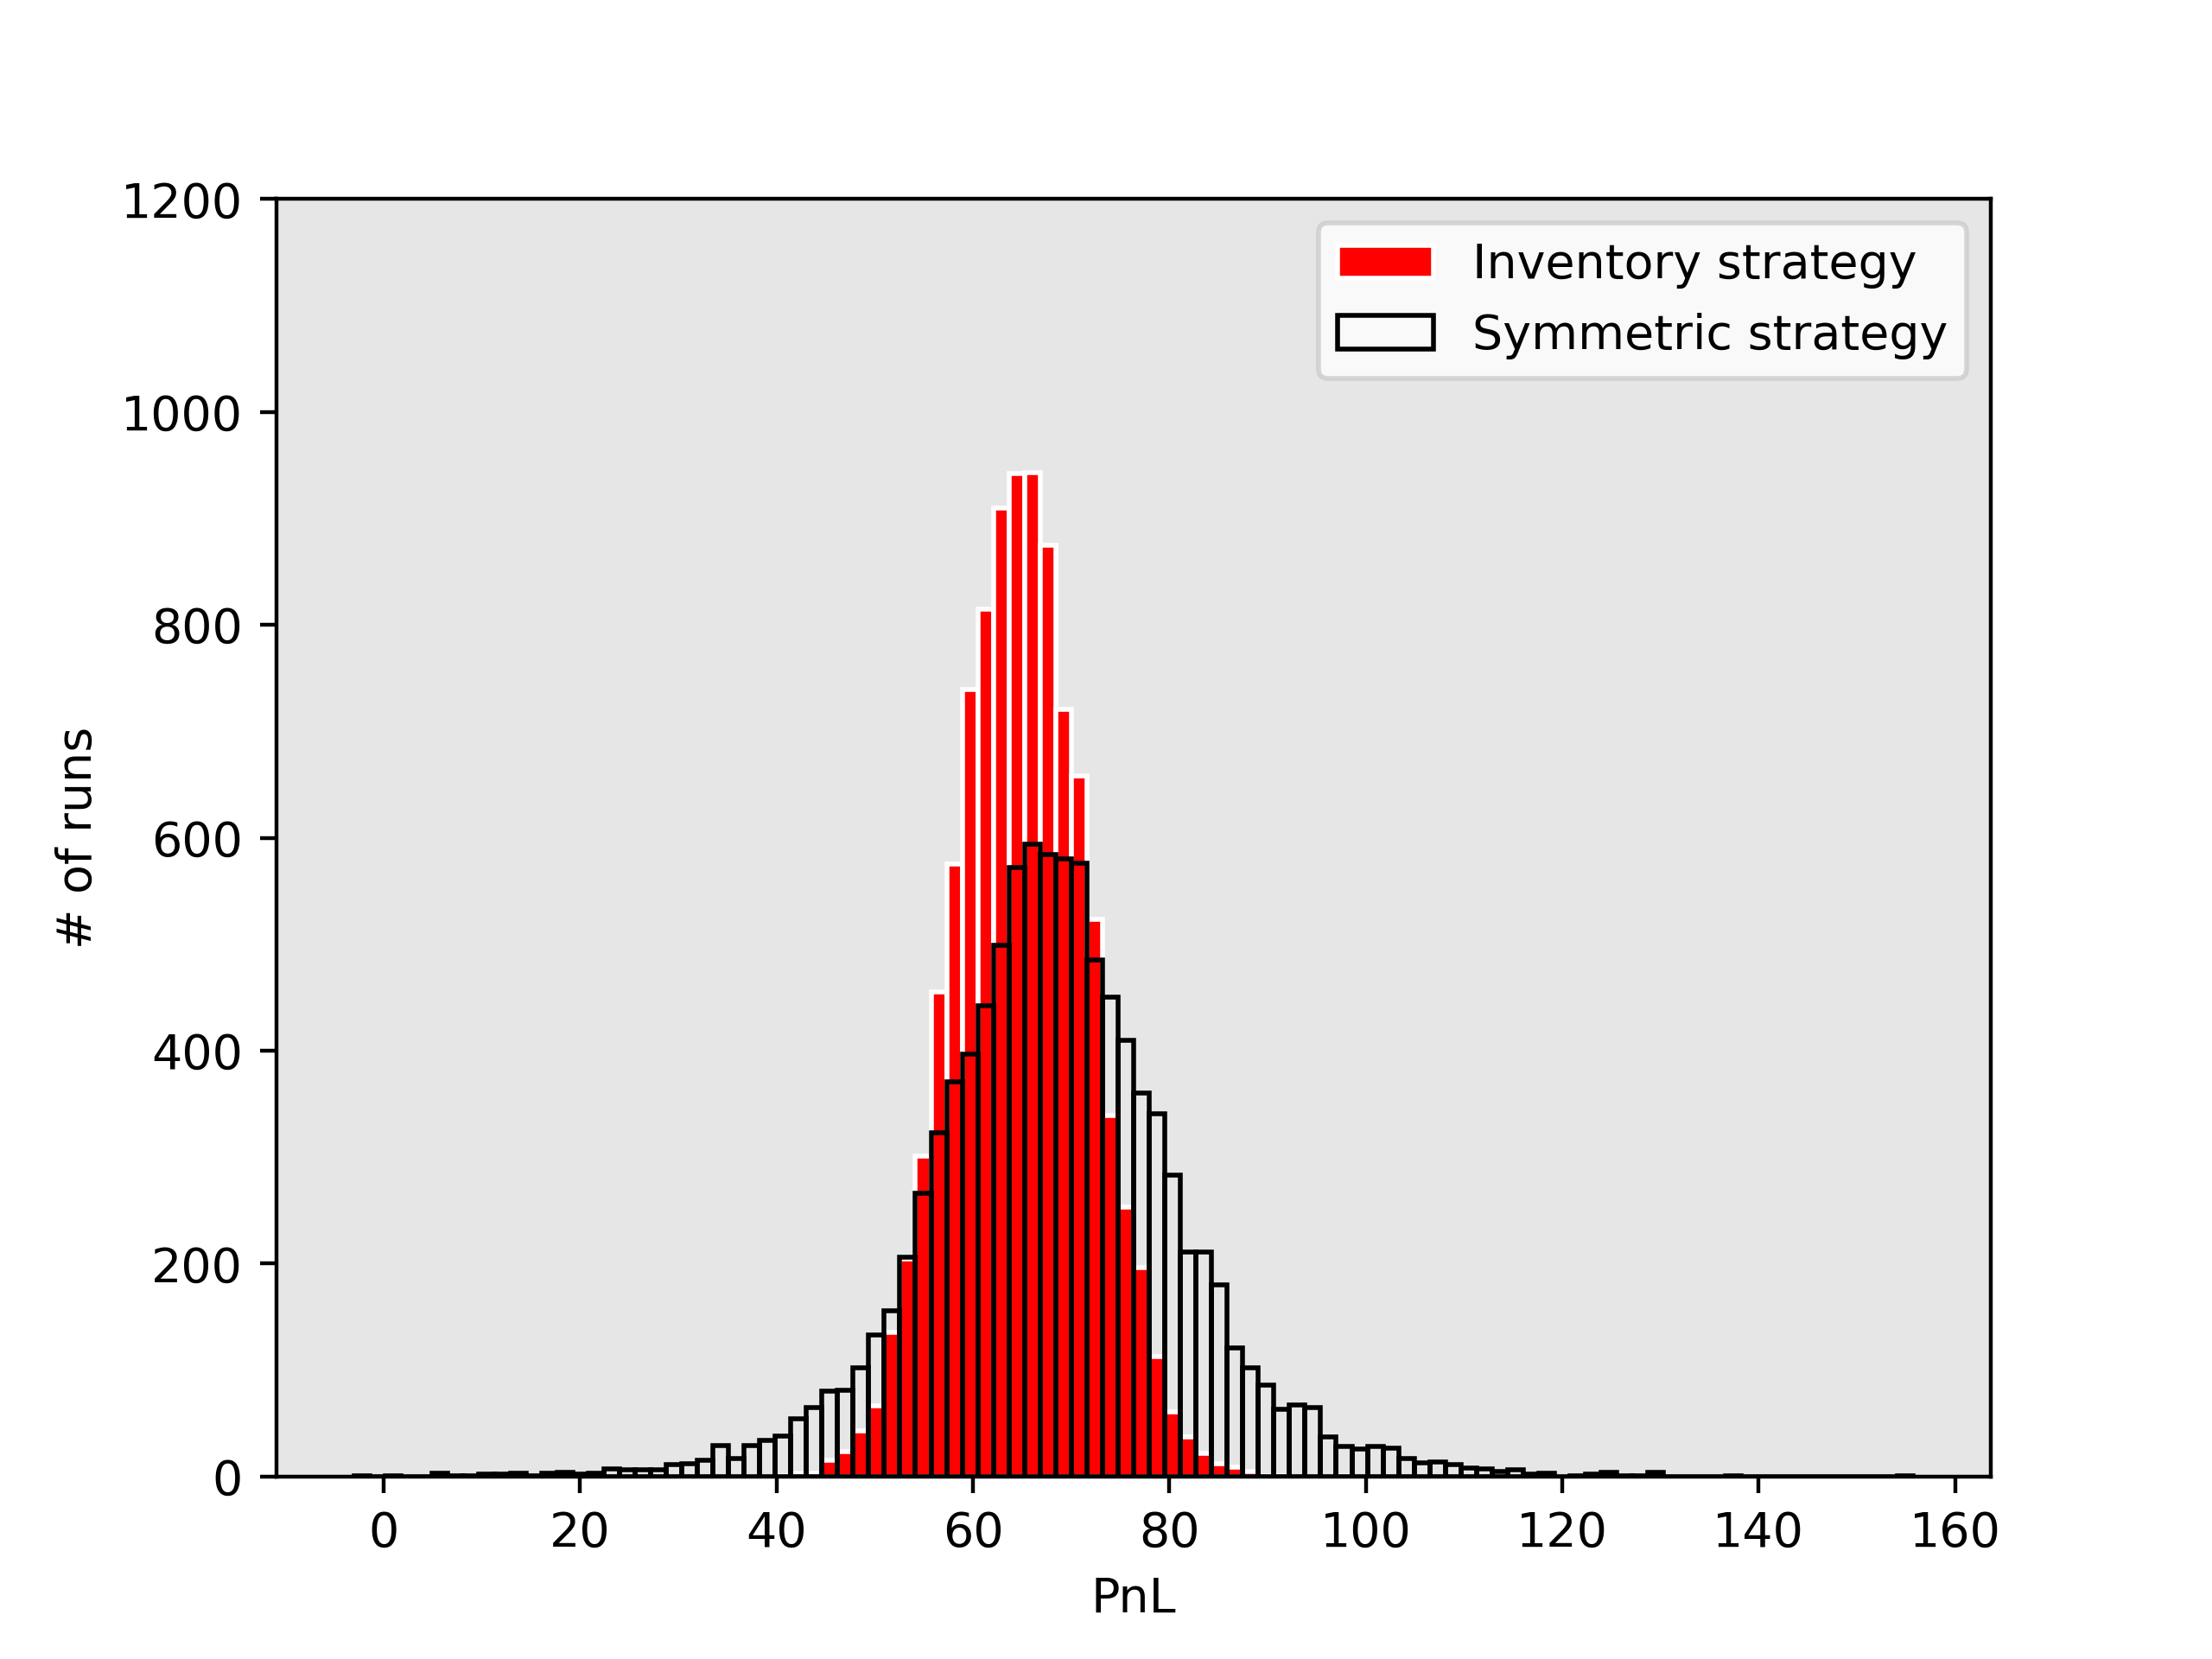
\includegraphics[scale=0.5]{gamma01.png}
        \caption{Results for $\gamma=0.1$}
        \label{fig:results-gamma01}
    \end{figure}

\begin{figure}
    \centering
        \begin{tabular}{ c c c c c c } 
            \hline
            Strategy & $\mu$ (Spread) & $\mu$ (Profit) & $\sigma$ (Profit) & $\mu$ (Final q) & $\sigma$ (Final q) \\ 
            \hline
            Inventory & 1.35 & 68.5 & 9.1 & 0.04 & 5.3 \\
            Symmetric & 1.35 & 68.6 & 13.8 & 0.04 & 8.6 \\
            \hline
        \end{tabular}
        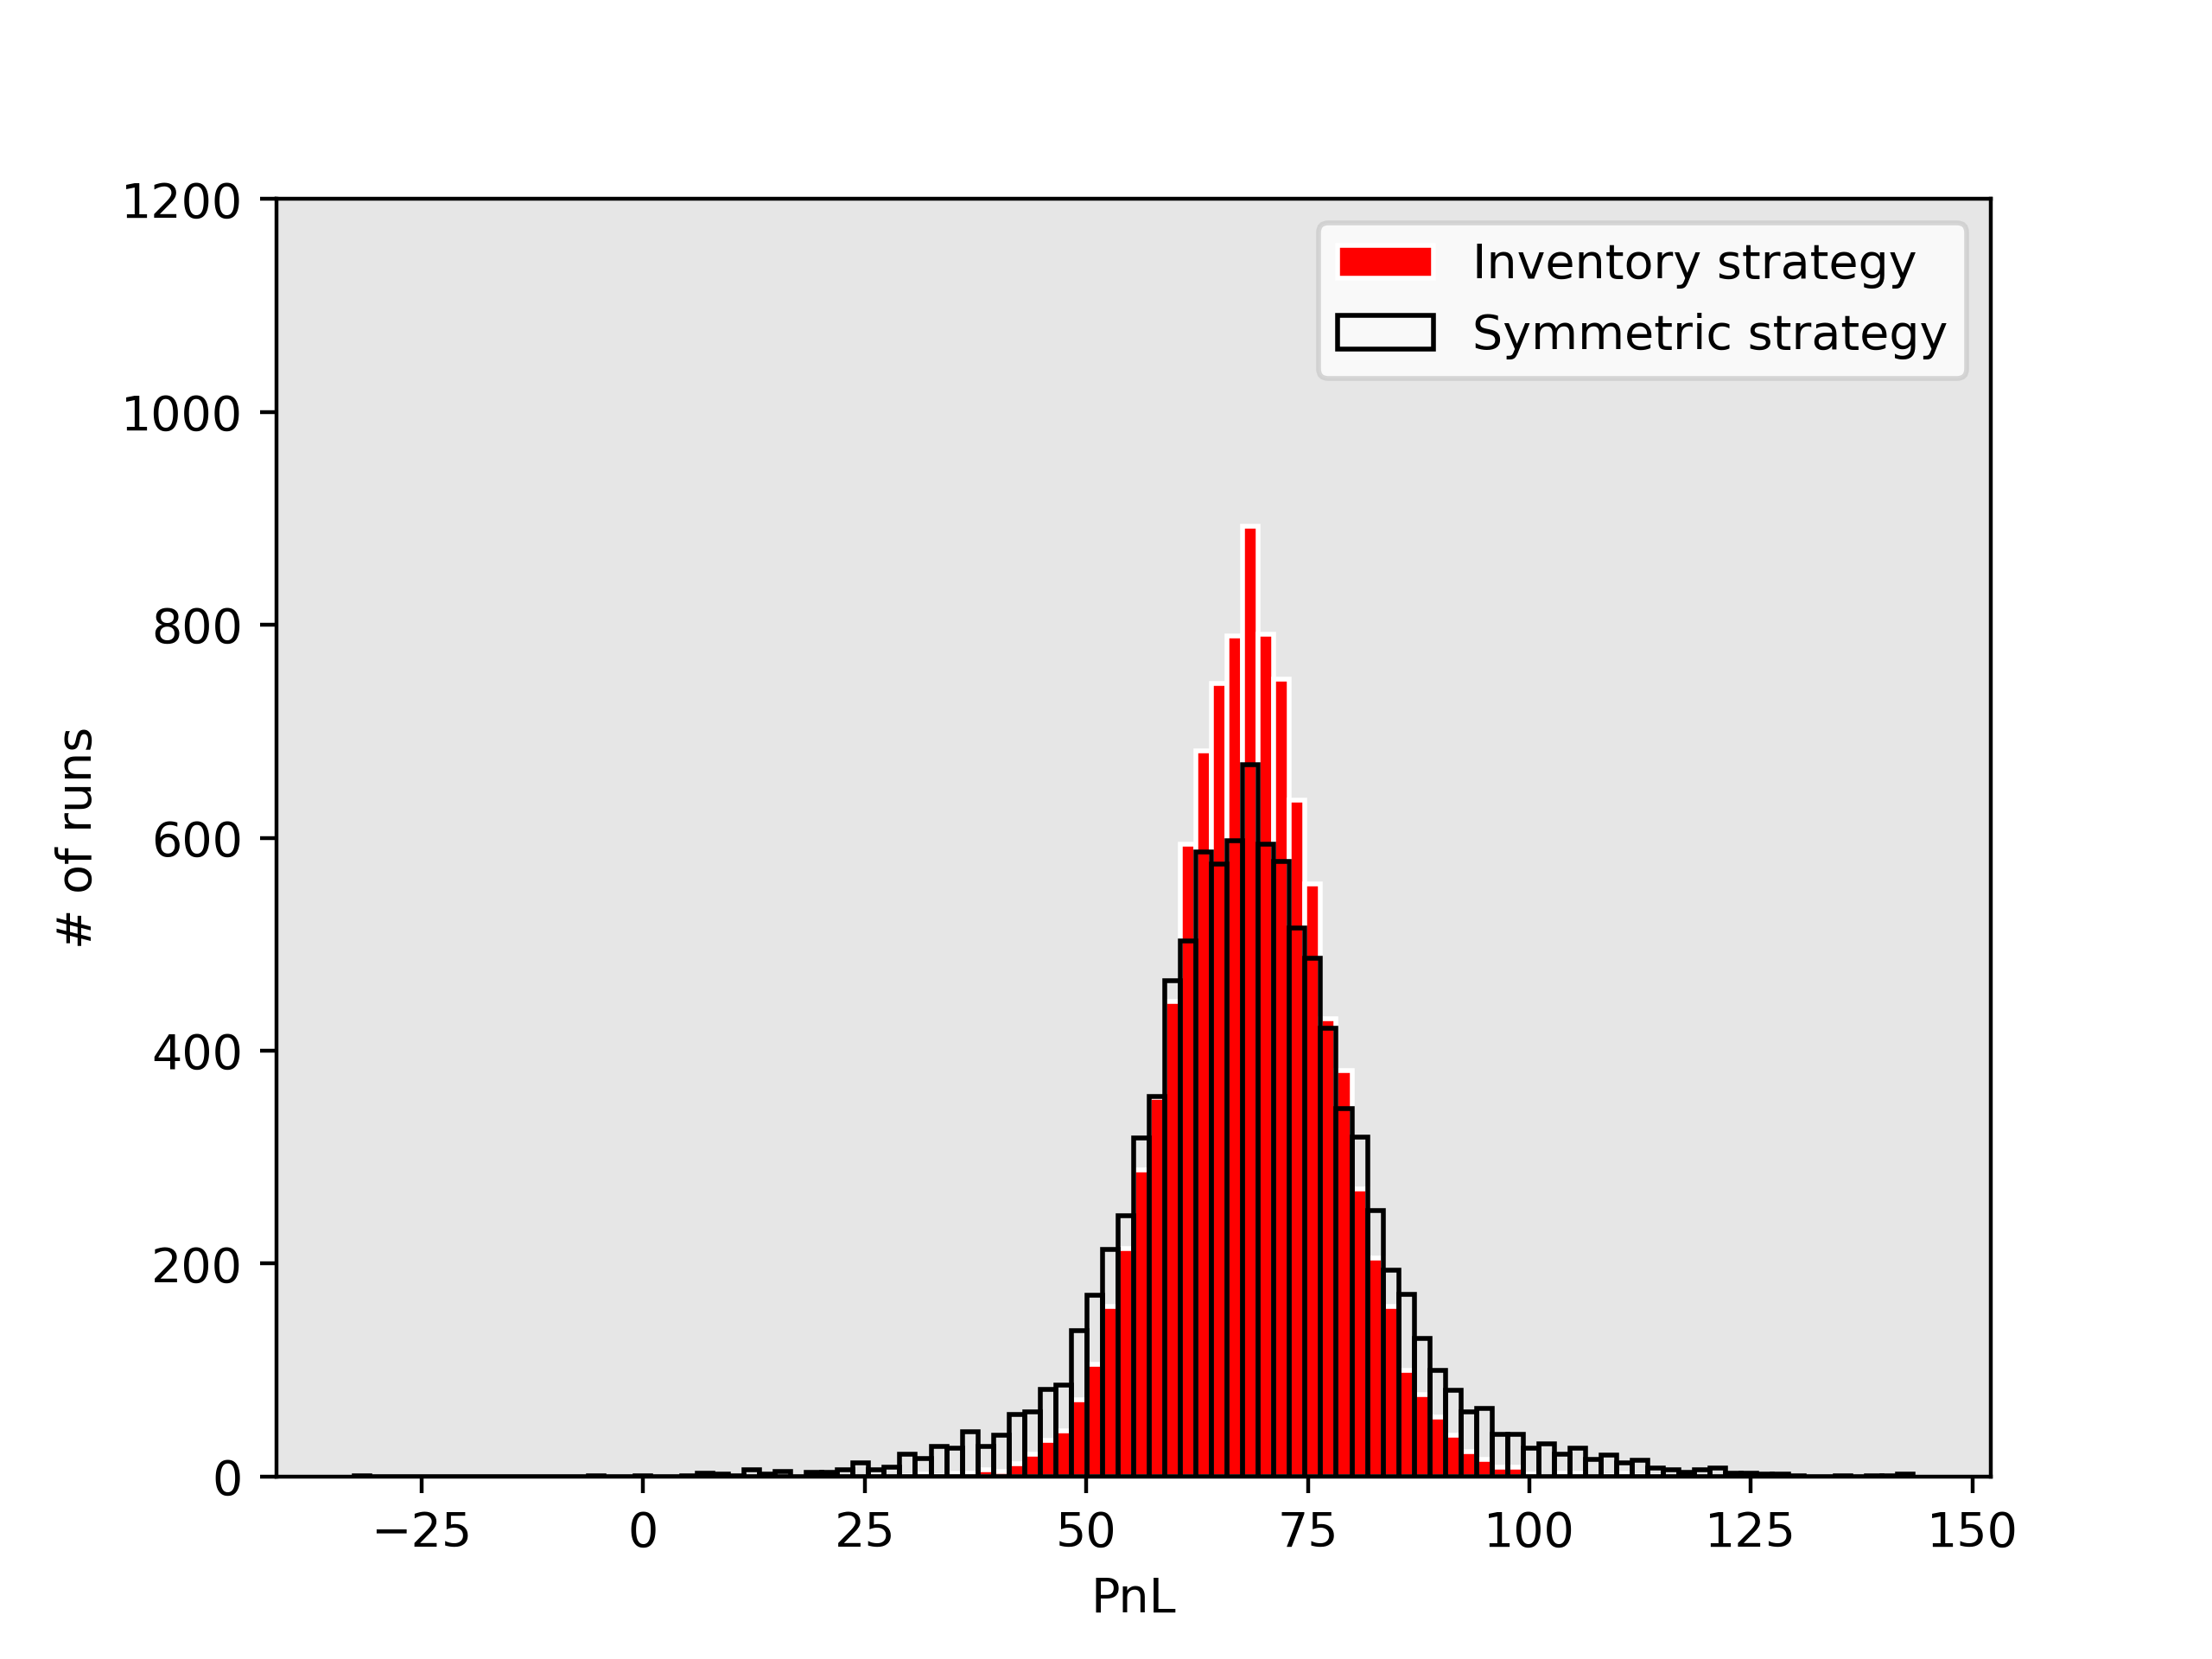
\includegraphics[scale=0.5]{gamma001.png}
        \caption{Results for $\gamma=0.01$}
        \label{fig:results-gamma001}
    \end{figure}

\section{Simulation of Extended Model for GBM}
\section{Estimation of Order Book Parameters for Real-World Data}
\section{Market Making in the Binance Order Book}